\numberwithin{equation}{section}

\subsection{Nondimensionalization}
%\begin{frame}
  %\frametitle{Outline}
  %\tableofcontents[ currentsection ]
%\end{frame}

\begin{frame}
\frametitle{Nondimensionalization}

The initial model is

  \begin{align*}
    \frac{dx}{dt} & = rx^2 \left(1-\frac{x}{K}\right) - \alpha xy - \frac{x^2 \gamma_\circ}{x+D}, \\
    \frac{dy}{dt} & = \rho y^2 \left(1-\frac{y}{L}\right) - \beta xy -\frac{y^2 \delta_\circ}{y+R}.
  \end{align*}
	
Let 
\begin{align*}
		& x \rightarrow A \hat{x} (s) \\
		& y \rightarrow B \hat{y} (s) \\
		& t \rightarrow \tau \cdot s
\end{align*}
When you substitute and group terms the system becomes nondimensionalized. 
\end{frame}

\begin{frame}
After making the following substitutions: \\
\begin{align*}
		A &= K, \\
		B &= L, \\
		\tau &= \frac{1}{rK}.	
\end{align*}

The nondimensionalized system is:

	\begin{align*}
		\frac{dx}{dt} &= x^2 (1-x) - \alpha xy - \frac{\gamma_\circ x^2}{x+D}, \\
    \frac{dy}{dt} &= \rho y^2 (1-y) - \beta xy -\frac{\delta_\circ y^2}{y+R}
	\end{align*}
\end{frame}

\begin{frame}{Phase Plane}

  \vfill
	
	When we start with the initial parameters $\alpha = .2, \beta = .2, \gamma = .8, \delta = .4, \rho = 1, R = 3$ and $D = 7$ this is our phase plane. 
  
	WE NEED TO CHANGE THIS PHASE PLANE. 
  \begin{columns}
    \column{.65\textwidth}
       \includegraphics[height=7cm]{img/typeIPhasePlane}
    \column{.35\textwidth}
    \begin{itemize}
    \item Four fixed points.
    \item Two are unstable.
    \end{itemize}
  \end{columns}
\end{frame}

\begin{frame}
 What happens if we change the parameters to $\gamma = .85$ and $\delta = .8$
\\
INSERT NEW PHASE PLANE. 
\end{frame}

\begin{frame}
 What happens if we change the parameters to $\alpha = .9, \beta = .2, \gamma = .8$ and $\delta = .4$
\\
INSERT NEW PHASE PLANE. 
\end{frame}

\begin{frame}
 What happens if we change the parameters to $\alpha = .5, \beta = .5, \gamma = .8$ and $\delta = .4$
\\
INSERT NEW PHASE PLANE. 
\end{frame}

\begin{frame}
 What happens if we change the parameters to $\alpha = .95, \beta = .95, \gamma = .8$ and $\delta = .4$
\\
INSERT NEW PHASE PLANE. 
\end{frame}

\begin{frame}{Noise}
		What happens if we add noise?
	\begin{align*}
		\frac{dx}{dt} &= x^2 (1-x) - \alpha xy - \frac{\gamma_\circ x^2}{x+D} + \text{``noise,''} \\
    \frac{dy}{dt} &= \rho y^2 (1-y) - \beta xy -\frac{\delta_\circ y^2}{y+R}+ \text{``noise.''}
	\end{align*}
\end{frame}

\begin{frame}{Additive Noise}
		If we add additive noise... 
	\begin{align*}
		\frac{dx}{dt} &= x^2 (1-x) - \alpha xy - \frac{\gamma_\circ x^2}{x+D} + \upsilon \frac{dW}{dt}, \\
    \frac{dy}{dt} &= \rho y^2 (1-y) - \beta xy -\frac{\delta_\circ y^2}{y+R}+ \kappa \frac{dB}{dt}.
	\end{align*}
\end{frame}

\begin{frame}{Proportional Noise}
		If we add proportional noise... 
	\begin{align*}
		\frac{dx}{dt} &= x^2 (1-x) - \alpha xy - \frac{\gamma_\circ x^2}{x+D} + \upsilon x \frac{dW}{dt}, \\
    \frac{dy}{dt} &= \rho y^2 (1-y) - \beta xy -\frac{\delta_\circ y^2}{y+R}+ \kappa y \frac{dB}{dt}.
	\end{align*}
\end{frame}




\begin{frame}
\frametitle{Heun's Method}
\begin{itemize}
\item Heun's method is a numerical procedure for approximating ordinary differential equations with a given initial value.
\item First you calculate the intermediate value $\tilde{y}_{i+1}$ and then the final approximation $y_{i+1}$ at the next generation point.
\end{itemize}

\begin{align*}
	\tilde{y}_{i+1} &= y_i + \Delta t \ f(t_i, y_i) \\
	y_{i+1} &= y_i + \frac{\Delta t}{2} \left[f(y_i,t_i) + f(\tilde{y}_{i+1}, t_{i+1})\right]
\end{align*}
\end{frame}


\begin{frame}
   \frametitle{Heun's Method vs. Euler's Method - Simulation}
For the DE $y'=r y$ on $[0,T]$,\\
\vspace{1em}
	%\hspace{1.5em} Heun's:$\hspace{1em} \tilde{y}_{i+1} = y_i + \Delta t \ f(t_i, y_i)$ \\
		\hspace{1.5em} Heun's:$ \hspace{1em} y_{i+1} = y_i + \frac{\Delta t}{2} \left[f(y_i,t_i) + f(\tilde{y}_{i+1}, t_{i+1})\right]$ \vspace{1em} \\
	\hspace{1.5em} Euler's:$\hspace{1em}\tilde{y}_{i+1} = y_i + \Delta t \ f(y_i, t_i)$ \\
\begin{columns}[t]
    \column{.5\textwidth} 
    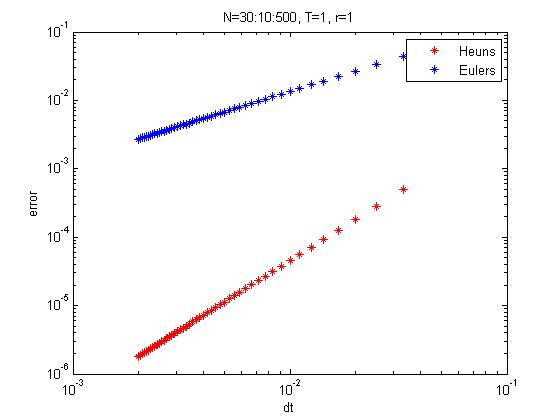
\includegraphics[width=6cm]{img/Heun500}
    \column{.5\textwidth}
    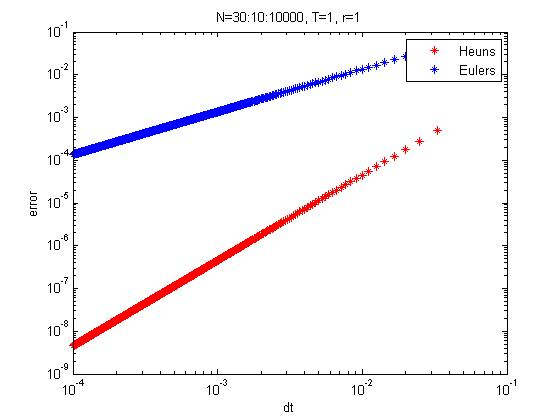
\includegraphics[width=6cm]{img/Heun10000}
  \end{columns}

\end{frame}
